\section{October 28, 2022}

\subsection{Simple Groups and Group Extensions}

\begin{definition}
\deflabel

$G$ is \ac{simple} if $G\neq \{1\}$ and the only normal subgroups of $G$ are $\{1\}$ and $G$.
\end{definition}

\begin{example}
\exlabel

$G = C_p$ is simple for all prime $p$.
\end{example}

\begin{definition}
\deflabel

Let $N$ be a normal subgroup in $G$. Then, $G$ is an \ac{extension} of $G/N$ by $N$. This extension is $\ac{split}$ if $G$ has a subgroup $H$ isomorphic to $G/N$ under the canonical map. Remember that the canonical map takes $g\mapsto gN$, so this says that there exists some subgroup of $G$ that maps to all cosets of $N$.
\end{definition}

Intuitively, extensions may seem equivalent to products (i.e., if $G$ is an extension of $Q$ by $N$, then $G$ is isomorphic to $Q\times N$). But, they're not. Consider the following examples. 

\begin{example}
\exlabel

Let $G = \ZZ$ and $N = 2\ZZ$. 
\end{example}
Then, we can say that $G$ is an extension of $G/N \cong C_2$ by $N$. This extension is not split, since there aren't any subgroups of $G$ isomorphic to $C_2$. In this case, $G \ncong C_2\times N$, since the former has a single generator, while the latter does not.

\begin{example}
\exlabel

Let $G = M_n$ and $N = O_n(\RR)$. 
\end{example}

Then, we can say that $G$ is a split extension of $G/N = \RR^n$ by $O_n(\RR)$. This extension is split, because the set of translations is isomorphic to $G/N$ under the canonical map. In this case, $G\ncong O_n(\RR)\times \RR^n$, since composition breaks the multiplication law. While they aren't a direct product, they are a \ac{semidirect product}.  

\subsection{Rotations of an icosahedron}

\begin{figure}[h]
\centering
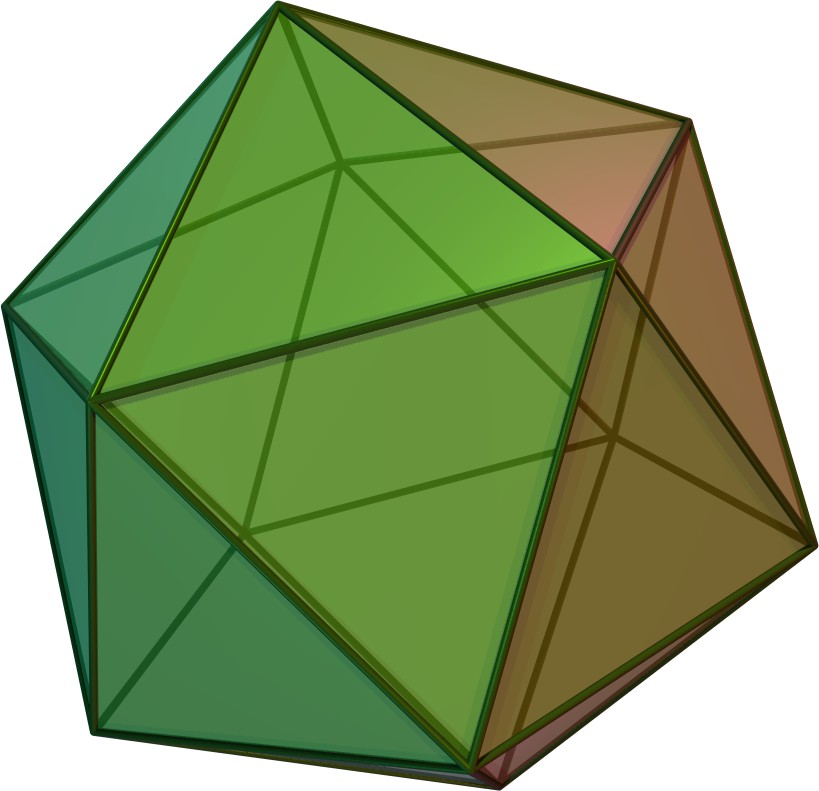
\includegraphics[width=4cm]{images/icosahedron.jpeg}
\end{figure}

Let $G\subseteq SO_3(\RR)$ be the group of rotations of an icosahedron. Recall that an icosahedron has $20$ faces, $30$ edges, and $12$ vertices. All faces are triangular and each vertex is the meeting of $5$ faces. 

To be explicit, when we say ``the group of rotations", what we mean is that we choose any axis of rotation through the center of the icosahedron, and then rotate the figure through some angle such that its image after rotation is the same as the preimage (i.e., the alignment of the icosahedron is the same as before). 

Now, we categorize the conjugacy classes of $G$. Recall that any conjugacy class is just a self-contained set of rotations that can be reached by some element in $G$. In other words, for any two rotations, if there is a rotation of the icosahedron that maps these two rotations together, they are in the same conjugacy class. 

\begin{itemize}
    \item The identity rotation. Conjugation of the identity always produces the identity again, so this is self contained.
    \item Any rotation that fixes a face. For these rotations, we choose our axis of rotation such that it goes through the center of our fixed face. In this case, this axis also goes through the center of the face opposite to our chosen face, so we have to consider pairs of opposite faces.
    
    There are $10$ pairs of opposite faces. Moreover, each face borders $3$ other faces, so there are two non-identity rotations per pair ($\pm 120^{\circ}$), giving us $20$ elements.
    
    This is self-contained, because regardless of our choice of perspective, the property that a rotation fixes a face is invariant. We must include both CW and CCW rotations, since for any pair of opposite faces $(A, B)$, a CW rotation for $A$ is a CCW rotation for $B$.
    \item Any rotation that fixes an edge. For these rotations, similar to the face rotations, we choose our axis of rotation such that it goes through the middle of our fixed edge. This axis will again go through the center of the edge opposite to our chosen edge, so we have to consider pairs of opposite edges. 
    
    There are $15$ pairs of opposite edges. For each of these pairs, there is one non-identity rotation ($180^{\circ}$) which swaps the vertices of our chosen edge, giving us $15$ elements. 
    \item Any rotation of $\pm 72^{\circ}$ that fixes a vertex. We choose our axis of rotation such that it goes through our chosen vertex. As before, this axis will also go through the vertex opposite our chosen vertex, so we need to consider pairs of vertices, of which there are $6$. For each vertex, there are four non-identity rotations that fix that vertex. For any pair of vertices $(A,B)$, a CW $72^{\circ}$ rotation for $A$ is the same as a CCW $72^{\circ}$ for $B$, so these are contained in the same conjugacy class. This gives us $2\cdot 6=12$ elements.
    \item Any rotation of $\pm 144^{\circ}$ that fixes a vertex. This gives us another $2\cdot 6 = 12$ elements. 
\end{itemize}

In sum, our class equation is given by 
\[\vert G\vert = 1 + 20 + 15 + 12 + 12.\]

This is confirmed by the orbit-stabilizer theorem. If we let $S$ be the set of faces, edges, or vertices of an icosahedron, the action of $G$ on $S$ gives $\vert G\vert = 20\cdot 3 = 30\cdot 2 = 12\cdot 5$.

\begin{theorem}
\thmlabel

$G$ is simple.
\end{theorem}
\begin{proof}
If $N$ is a normal subgroup of $G$, then $gN=Ng\implies N = gNg^{-1}$, so $N$ must be a union of conjugacy classes. This implies that $\vert N\vert$ is equal to the sum of the numbers in some subset of $\{1,12,12,15,20\}$. But since we also must have $\vert N\vert \mid \vert G\vert$, this forces $\vert N\vert = 1$ or $\vert N\vert = 60$, so $G$ is simple.
\end{proof}

\begin{theorem}
\thmlabel

$G\cong A_5$.
\end{theorem}

This is Theorem $7.4.4$ in Artin. 
\begin{figure}[h]
    \centering
    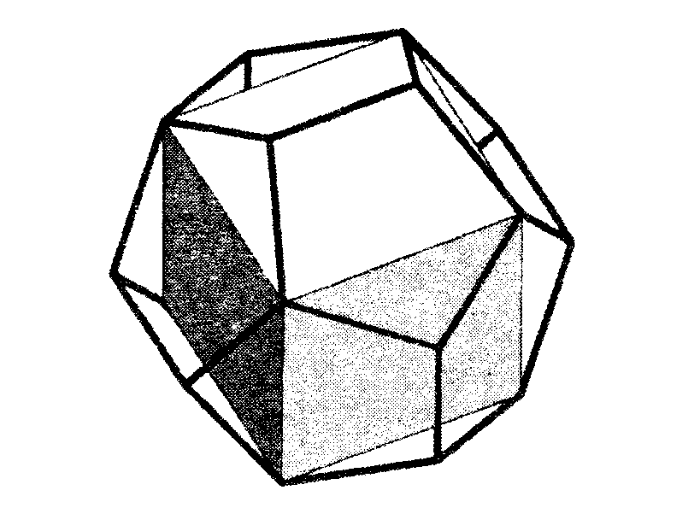
\includegraphics[width = 5cm]{images/inscribed_cube.png}
\end{figure}
\begin{proof}
The basic idea is to use the fact that there are five ways to inscribe a cube inside of an icosahedron. Because of duality, we can consider a dodecahedron instead (refer to the image above from Artin to help visualize). For any pentagonal face $ABCDE$, there are five ways to align an edge of the cube with diagonal vertices (i.e., $AC$, $BD$, $CE$, $DA$, $EB$). This completely determines the possible ways to inscribe a cube inside of the dodecahedron, since each edge of the cube (of which there are $12$) lies on exactly one face of the dodecahedron (of which there are also $12$).

Proposition $17.2$ then gives a homomorphism $\varphi$ from $G$ to $S_5$ (the associated permutation representation). The kernel of this homomorphism is trivial, since all kernels are normal subgroups, and $G$ is simple (the kernel can't be $G$, otherwise our homomorphism would do nothing).

This implies that $\varphi$ is injective, so it determines an isomorphism from $G$ to a subgroup of $S_5$. Now, restrict the sign homomorphism $S_5\rightarrow \{\pm 1\}$ to $G$. If it was surjective, then the kernel would have order $30$, which is not possible, since $G$ is simple. So $G$ must be a subgroup of $A_5$, which is the preimage of $+1$ under the sign homomorphism, but since they have the same size, they're the same group!
\end{proof}

There turns out to be broad categorization of simple groups.
\begin{theorem}
\thmlabel

There are four main categories of simple groups:
\begin{itemize}
    \item $C_p$, with $p$ prime
    \item $A_n$, for $n\geq 5$
    \item ``groups of Lie type"
    \item $26$ sporadic groups
\end{itemize}
\end{theorem}

Prof. Cohn says that even he doesn't fully know the proof for this Theorem, so we won't be going over it in class. 